\documentclass[11pt]{jsk-thesis}

%レイアウト補正
%\usepackage{layout}
%\setlength \voffset {-1.0cm}
%\setlength \hoffset {-1.2cm}
%\setlength \textwidth {17cm}
%\setlength \textheight {24cm}

%パッケージ読み込み
\usepackage[dvipdfmx]{graphicx}
\usepackage[dvipdfmx]{color}
\usepackage{booktabs}
\usepackage{amsmath}
\usepackage{amssymb}
\usepackage{bm}
\usepackage{url}
\usepackage{otf}

%コマンド定義
%表の日付のフォントサイズ変更
\newcommand{\tdate}[1]{\scriptsize{#1}}
%単位"°"
%%\newcommand{\degree}[1]{#1^{\circ}}
%微分演算子関係
\newcommand{\dd}{\mathrm{d}}
\newcommand{\diff}[2]{\frac{\mathrm{d}#1}{\mathrm{d}#2}} %常微分
\newcommand{\diffline}[2]{\mathrm{d}#1/\mathrm{d}#2} %文章中での常微分
\newcommand{\ddiff}[3]{\frac{\mathrm{d}^#1 #2}{\mathrm{d} #3^#1}} %高階常微分
\newcommand{\ddiffline}[3]{\mathrm{d}^#1 #2/\mathrm{d} #2^#1} %文章中での高階常微分
\newcommand{\pdiff}[2]{\frac{\partial #1}{\partial #2}} %偏微分
\newcommand{\pddiff}[3]{\frac{\partial^#1 #2}{\partial #3^#1}} %高階偏微分
\newcommand{\non}[1]{#1^{*}} %無次元化変数

%関数
\newcommand{\erf}{\mathrm{erf}}

%その他
\newcommand{\myfig}[5]{
  \begin{figure}[#1]%
    \begin{center}%
      \includegraphics[width=#2]{#3}%
      \caption{#4}%
      \label{fig:#5}%
    \end{center}%
  \end{figure}%
}
%% \newcommand{\figref}[1]{Fig.\ref{fig:#1}}
%% \newcommand{\seclabel}[1]{\label{sec:#1}}
%% \newcommand{\secref}[1]{第{\bf\ref{sec:#1}}節}

\newcommand{\unit}[1]{\,[\mathrm{#1}]}

%見出し変更
\renewcommand{\figurename}{Fig.}
\renewcommand{\tablename}{Table}



\usepackage{ikuo}%%便利コマンド集.

\usepackage[dvipdfmx]{hyperref}  % 目次や参考文献をリンクにする。
\usepackage{pxjahyper} %% これを入れるとしおりが文字化けしない。out2uniが不要になる。
%% \hypersetup{bookmarksnumbered=true}
\hypersetup{colorlinks=true}
\hypersetup{linkcolor=black}
%% \hypersetup{linkbordercolor=black}
\hypersetup{urlcolor=black}
%% \hypersetup{urlbordercolor=black}
\hypersetup{citecolor=black}
%% \hypersetup{citebordercolor=black}

\usepackage{url} % \url のために必要。パッケージが無い人は探して入れる。
%% \url{http://nile.ulis.ac.jp/~yuka/}のようにして使う。

\newcommand{\FIGDIR}{./fig}        %図を置くディレクトリを指定する


\date{令和6年度卒業論文}
\title{卒論執筆に関する研究}
\author{指導教員 水内 郁夫 准教授 \\
\ \\
東京農工大学 \\
工学部 機械システム工学科 \\
\ \\
平成32年度入学\\
12345678\\
{\bf 山田 太郎}}

\begin{document}
\setlength{\baselineskip}{20pt}
\maketitle
\tableofcontents

%%各章は別ファイルにして以下にinculudeすると良い.
\chapter[序論]%
        {序論}

        \figb{photo.jpg}{width=0.75\hsize}{図1}%

        \fig{fig1.eps}{width=.9\hsize}{何かの図}%

        \section{研究の背景と目的}
        \seclabel{intro}

        投擲動作を行うスポーツは数多く存在するが、野球と砲丸投げのように競技によって投
        擲フォームは異なり、さらに同一競技内であっても個人によって投擲フォームは異なる。
        競技や個人によって投擲フォームが異なる要因として、投擲物や身体といった投擲フォー
        ムに関連するパラメータの違いが挙げられる。
        具体的なパラメータとして、投擲物は重さや大きさ、身体は慣性や各部位のサイズ等がある。
        これまで投擲フォームに関する研究例として、眞田の野球におけるオーバーハンドスローとサイドハンドスロー
        の球速の比較、大室らの野球における足の踏み出し幅による投球速度の比較、黒松らの砲丸投げグライド投法における投擲フォーム改善前後の飛距離の比較などがある。
        投擲フォームは球速や投擲物の飛距離等の、スポーツにおける総合性能に大きな影響を及ぼす。
        また、投擲に関する総合性能の研究例として、蔭山らの野球における年齢による体格や背筋力と投球速度の関係、
        高橋らの野球における肩関節と股関節の可動域・筋力と投球速度の関係、坪井らの砲丸投げにおける
        投射速度・投射角と飛距離の関係などがある。スポーツにおいて総合性能向上は最も重要な要素の一つである。
        これらの研究はある一つの競技に特定した研究である。しかし、さまざまなスポーツに応じた投擲フォームがどのような戦略
        の基で成立しているのかに関する汎用的な理論は確立されていない。
        そこで、本研究ではシミュレーションにおいてさまざまなパラメータに応じた投擲フォームを導出・比較することで、さまざまな投擲フォームの戦略を検討・考察・議論することを目的とする。
        対象となる投擲フォームは、遠投を行うための投擲フォームである。遠投は投射角と手先速度の二つの要素が影響し、それぞれのバランスが求められる。\\
        研究室が散らかっている(\figref{photo.jpg}参照)ので、片付けるロボットが欲
        しい。

        この図(\figref{fig1.eps})はなんだろう?

        \secref{intro}ではほげほげ。

        こういう研究\cite{Ikuo:doctor}もありました。

        ああいう研究\cite{Hondo:JRSJ2011}もありました。

        bibファイルでは、著者名(author=)は、
        「苗字 名前 and 苗字 名前 and 苗字 名前」
        のようにするんですよ\cite{Mizuuchi:RSJ2015-baneoid}。
        間は全部半角スペースですよ。

        \section{従来研究}

        \begin{table}[tb]
          \tablabel{hogehoge}
          \begin{center}
            \caption{試しに作った表}
            \begin{tabular}{l|c|r|r}
              \hline
              項目 & 数値 & コメント & 備考 \\
              \hline
              a & 10.0 & こめんとしがたい & どうすべ?\\
              b & 20.0 & こめんとしがたい & どうすべ?\\
              c & -100.0 & こめんとしがたい & どうすべ?\\
              \hline
            \end{tabular}
          \end{center}
        \end{table}

        \tabref{hogehoge}に、何かの表を示す。

        \section{本論文の構成}

\chapter[図の貼り方および表,式の書き方]{図の貼り方および\\表,式の書き方 }

\section{図の貼り方}
\seclabel{fig}

\subsection{基本的な図の貼り方}
図を貼る際には例えば以下のようにする.
\begin{figure}[t]%
  \begin{center}%
    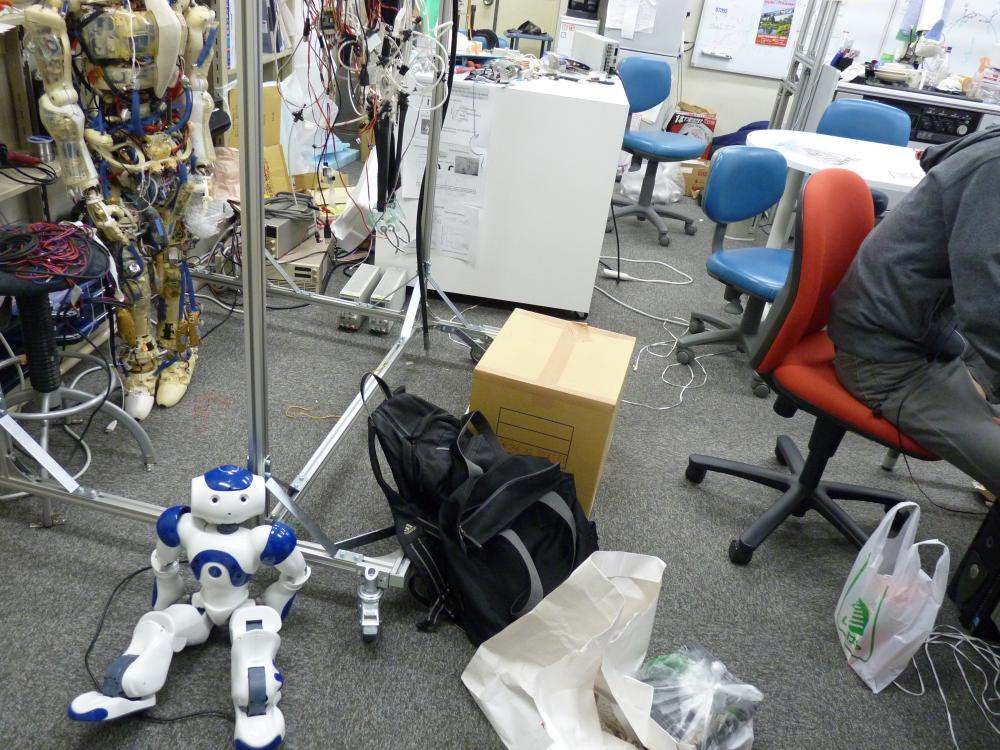
\includegraphics[width=0.50\hsize]{\FIGDIR/photo.jpg}%
    \caption{図の貼り方}%
    \label{fig:lab}%
  \end{center}%
\end{figure}%
図\ref{fig:lab}はこのようにして貼られた図である.
図に対して言及するときはこのようにrefコマンドを使う.
refコマンドの引数を,図を貼った時のコマンド群中のlabelコマンドの引数と対応させることで,意図した図に対してrefすることができるのである.

さて,先ほどの図の貼り方はちょっとめんどくさい.
大体,たかが図を一枚貼るためにこんな数行使った処理をいちいち書いてられないし,ソースコードのスペース的にもたくさん消費してしまってアホみたいである.
そのあたりを解決するのが,figコマンドである.
(figコマンドはいわば自作関数で,ikuo.styの中に定義されている.)
figコマンドを使うと,下記のように図を貼ることができる.
\fig{photo.jpg}{width=.50\hsize}{figコマンドを使って貼った図}
\figref{photo.jpg}はfigコマンドを使って貼った図である.
そして,今,気づいただろうか.
今のrefはただのrefではなく,figrefコマンドを使ってrefを行ったものである.
(figrefコマンドもfigコマンド同様にikuo.styの中で定義されている.)
figrefコマンドを使うと,いちいち「図」とか「fig.」とかをrefコマンドの前に書く必用がなくなり,便利である.
更に,「図」でなく「fig.」として参照するように変更する必用が生じた時にも,ikuo.styの中のfigrefコマンドの定義箇所にて変更をするだけで文書全体に変更が行われるのでとても有用であり,figrefコマンドを使わないのは愚かしい行為である.


\subsection{figに関連する便利コマンド}

figコマンドには残念ながら,図の位置を指定する引数が存在しない.
figコマンドの定義を見ると,位置指定オプションは[tbp]となっており,ページ上端,下端,まるまる1ページ,という優先度で位置が指定されることがわかる.
どうしてもページ下端に図を貼りたいんだ,という時にはfigbコマンドが用意されている.
\figb{photo2.jpg}{width=.50\hsize}{figbコマンドを使って貼った図}
\figref{photo2.jpg}はfigbコマンドを使って貼った図である.

どうしても位置を自分で指定したい,という場合はfigposコマンドを使う.
figposコマンドは第4引数が位置指定オプションに反映されるため,下記のように使うことができる.
\figpos{photo3.jpg}{width=.50\hsize}{figposコマンドを使って貼った図}{t}
\figref{photo3.jpg}はfigposコマンドを使って貼った図である.

上記各コマンドと合わせ,定義されているfig関連のコマンドを以下にまとめておく.
\begin{itemize}
\item fig\\
  図を貼るときに使う一番基本的なコマンド.
  位置指定は[tbp]となる.
  
\item twofigs\\
  2枚の図を立てに並べて貼るときに使うコマンド.
  キャプションは1つだけつき,ラベルは最初の図のファイル名になる.
  位置指定は[tbp]となる.
  
\item figthroug\\
  複数段組の文書中で,段組をぶちぬいて図を貼るときに使うコマンド.
  
\item figb\\
  ページ下端に図を貼るときに使うコマンド.
  
\item figpos\\
  任意の位置を指定して図を貼るときに使うコマンド.
  
\item doublefig\\
  2枚の図を横に並べて貼るときに使うコマンド.
  キャプションは1つだけつき,ラベルは最初の図のファイル名になる.
  位置指定は[tb]となる.
  
\item doublefigt\\
  doublefigコマンドと同様だが,ページ上端に図を貼るとき専用のコマンド.
  具体的には図の上側にスペースを入れずに貼ることができる.
  
\item doublefigb
  doublefigコマンドと同様だが,ページ下端に図を貼るとき専用のコマンド.
  
\item doublefigthrough\\
  doublefigコマンドと同様だが,複数段組の文章中で段組をぶちぬいて図を貼るときに使うコマンド.
  位置指定は[t]となる.
  
\item triplefig\\
  3枚の図を横に並べて貼るときに使うコマンド.
  キャプションは1つだけ表示され,ラベルは最初の図のファイル名になる.
  位置指定は[tbp]となる.
  
\item triplefigthrough\\
  triplefigコマンドと同様だが,複数段組の文章中で段組をぶちぬいて図を貼るときに使うコマンド.
  位置指定は[tbp]となる.
  
\end{itemize}


\section{表と式の書き方}
\seclabel{table_equation}

\subsection{表の書き方}
表を書くときには以下のようにする.
\begin{table}[tb]
  \label{sample}
  \begin{center}
    \caption{各人データ}
    \begin{tabular}{l|c|c|r}
      \hline
      名前 & 身長[cm] & 体重[kg] & 備考 \\
      \hline
      Y.M & 1800 & 60 & \\
      Y.M & 170 & 10 & \\
      Y.M & 170 & 60 & はげ\\
      \hline
    \end{tabular}
  \end{center}
\end{table}
表\ref{sample}は最も基本的な表の書き方の例である.
ソースコードを見ればわかる通り,この中ではlabelコマンドが使われているのだが,より便利なコマンドとしてtablabelが用意されている.
tablabelコマンドは表に対するラベルであるという情報をを自動的に付与してくれるため,これを用いることで図や式に対するラベルとごっちゃになるという問題を防ぐことができる.
同様のコマンドとしてfiglabel(図に対するラベル),equlabel(式に対するラベル),chaplabel(章に対するラベル),seclabel(節に対するラベル),subseclabel(小節に対するラベル)などが存在するので使うと良い.
\secref{fig}において用いたfigだとかtwofigだとかいった便利コマンドにおいてはその中でfiglabelが使用されている.

tablabelコマンドを用いた表は以下のようになる.
\begin{table}[tb]
  \tablabel{sample2}
  \begin{center}
    \caption{各人データ}
    \begin{tabular}{l|c|c|r}
      \hline
      名前 & 身長[cm] & 体重[kg] & 備考 \\
      \hline
      Y.M & 1800 & 60 & \\
      Y.M & 170 & 10 & \\
      Y.M & 170 & 60 & はげ\\
      \hline
    \end{tabular}
  \end{center}
\end{table}
\tabref{sample2}のようにtablabelを用いて表を書くと,tabrefコマンドを使うのが便利になる.
tabrefコマンドはfigrefコマンドのように自動で「図」とか「table」とかをつけてくれる便利コマンドである.

表に関しては特にこれ以上ローカルなコマンドとかないので,あとは研究室wikiを見るなりネットで情報探すなりして自分の書きたい表を書けるようになってください.


\subsection{式の書き方}
式は例えば以下のように書く.
\begin{eqnarray}
  \equlabel{hoge}
  hoge=hage
\end{eqnarray}

式に関してここで述べるべきことは表に関するそれとほぼ同様であり,つまりequlabelおよびequrefを使うべきであるという点のみである.
\equref{hoge}はequlabelを使ってラベル付されており,本文章冒頭のrefはequrefを用いて行われている.
式の書き方に関するそれ以外の情報は研究室wikiなりネット上で情報探すなりしてください.


\addcontentsline{toc}{chapter}{謝辞}
\markboth{謝辞}{謝辞}
\chapter*{謝辞}
本論文は,筆者が東京農工大学大学院生物システム応用科学府生物機能システム科学専攻博士前期課程に在学中に行った研究をまとめたものです.\\
 本論文をまとめるにあたり,丁寧なご指導ご鞭撻を賜った東京農工大学生物システム応用科学府生物機能システム科学専攻 水内郁夫教授に深く感謝の意を表します.水内先生には貴重なご意見や適切なご指導をいただき,充実した研究生活を送ることができました.また,目上の方に対する礼儀はもちろん,研究報告会等私の今後の人生に重要な知識・経験をご教授していただく機会も多く,大変貴重な日々でした.改めて心より感謝申し上げます.\\
 森下克幸助教にも深く感謝の意を表します.森下先生には普段から積極的にコミュニケーションを取っていただき,その都度貴重なご意見をいただきました.お気遣いいただいたこともあり,研究をより充実したものにしていただきました.\\
 本学在籍時に関わった研究室のメンバーには大変お世話になりました.特に同期の長田京右さん,菅野公景さん,高橋龍乃介さん,山本雄大さんは共に過ごす時間も長く大変お世話になりました.長田くんとは研究活動外でも共に行動することが多く,他愛もない会話をしていつも楽しませてくれました.菅野くんは頼りになる研究時と研究外のギャップが大きく,いつも笑わせてくれました.高橋くんとは話すたびにふざけ合って,疲れを吹き飛ばしてくれました.山本君は研究テーマも近く,また夜中に研究室で話をしたりして切磋琢磨することができました.また,先輩の赤羽聖さんにも大変お世話になりました.研究時の研究外でも頼れる兄貴分的な存在であり,いつも支えていただきました.また,M1とB4の後輩たちにも大変お世話になりました.先輩後輩の垣根を越えて交流をしてくれたおかげで,研究生活が一層楽しいものになりました.これからもより一層頑張ってください.\\
 最後に,学費の援助,生活の支援をしてくれた両親に,心より感謝申し上げます.学生生活で多くの経験をすることができたのも両親による支えがあったからであると感じています.本当にありがとうございました.


\addcontentsline{toc}{chapter}{参考文献}
\markboth{参考文献}{参考文献}
\bibliographystyle{junsrt}
\bibliography{reference}

\end{document}
